\documentclass[1p]{elsarticle_modified}
%\bibliographystyle{elsarticle-num}

%\usepackage[colorlinks]{hyperref}
%\usepackage{abbrmath_seonhwa} %\Abb, \Ascr, \Acal ,\Abf, \Afrak
\usepackage{amsfonts}
\usepackage{amssymb}
\usepackage{amsmath}
\usepackage{amsthm}
\usepackage{scalefnt}
\usepackage{amsbsy}
\usepackage{kotex}
\usepackage{caption}
\usepackage{subfig}
\usepackage{color}
\usepackage{graphicx}
\usepackage{xcolor} %% white, black, red, green, blue, cyan, magenta, yellow
\usepackage{float}
\usepackage{setspace}
\usepackage{hyperref}

\usepackage{tikz}
\usetikzlibrary{arrows}

\usepackage{multirow}
\usepackage{array} % fixed length table
\usepackage{hhline}

%%%%%%%%%%%%%%%%%%%%%
\makeatletter
\renewcommand*\env@matrix[1][\arraystretch]{%
	\edef\arraystretch{#1}%
	\hskip -\arraycolsep
	\let\@ifnextchar\new@ifnextchar
	\array{*\c@MaxMatrixCols c}}
\makeatother %https://tex.stackexchange.com/questions/14071/how-can-i-increase-the-line-spacing-in-a-matrix
%%%%%%%%%%%%%%%

\usepackage[normalem]{ulem}

\newcommand{\msout}[1]{\ifmmode\text{\sout{\ensuremath{#1}}}\else\sout{#1}\fi}
%SOURCE: \msout is \stkout macro in https://tex.stackexchange.com/questions/20609/strikeout-in-math-mode

\newcommand{\cancel}[1]{
	\ifmmode
	{\color{red}\msout{#1}}
	\else
	{\color{red}\sout{#1}}
	\fi
}

\newcommand{\add}[1]{
	{\color{blue}\uwave{#1}}
}

\newcommand{\replace}[2]{
	\ifmmode
	{\color{red}\msout{#1}}{\color{blue}\uwave{#2}}
	\else
	{\color{red}\sout{#1}}{\color{blue}\uwave{#2}}
	\fi
}

\newcommand{\Sol}{\mathcal{S}} %segment
\newcommand{\D}{D} %diagram
\newcommand{\A}{\mathcal{A}} %arc


%%%%%%%%%%%%%%%%%%%%%%%%%%%%%5 test

\def\sl{\operatorname{\textup{SL}}(2,\Cbb)}
\def\psl{\operatorname{\textup{PSL}}(2,\Cbb)}
\def\quan{\mkern 1mu \triangleright \mkern 1mu}

\theoremstyle{definition}
\newtheorem{thm}{Theorem}[section]
\newtheorem{prop}[thm]{Proposition}
\newtheorem{lem}[thm]{Lemma}
\newtheorem{ques}[thm]{Question}
\newtheorem{cor}[thm]{Corollary}
\newtheorem{defn}[thm]{Definition}
\newtheorem{exam}[thm]{Example}
\newtheorem{rmk}[thm]{Remark}
\newtheorem{alg}[thm]{Algorithm}

\newcommand{\I}{\sqrt{-1}}
\begin{document}

%\begin{frontmatter}
%
%\title{Boundary parabolic representations of knots up to 8 crossings}
%
%%% Group authors per affiliation:
%\author{Yunhi Cho} 
%\address{Department of Mathematics, University of Seoul, Seoul, Korea}
%\ead{yhcho@uos.ac.kr}
%
%
%\author{Seonhwa Kim} %\fnref{s_kim}}
%\address{Center for Geometry and Physics, Institute for Basic Science, Pohang, 37673, Korea}
%\ead{ryeona17@ibs.re.kr}
%
%\author{Hyuk Kim}
%\address{Department of Mathematical Sciences, Seoul National University, Seoul 08826, Korea}
%\ead{hyukkim@snu.ac.kr}
%
%\author{Seokbeom Yoon}
%\address{Department of Mathematical Sciences, Seoul National University, Seoul, 08826,  Korea}
%\ead{sbyoon15@snu.ac.kr}
%
%\begin{abstract}
%We find all boundary parabolic representation of knots up to 8 crossings.
%
%\end{abstract}
%\begin{keyword}
%    \MSC[2010] 57M25 
%\end{keyword}
%
%\end{frontmatter}

%\linenumbers
%\tableofcontents
%
\newcommand\colored[1]{\textcolor{white}{\rule[-0.35ex]{0.8em}{1.4ex}}\kern-0.8em\color{red} #1}%
%\newcommand\colored[1]{\textcolor{white}{ #1}\kern-2.17ex	\textcolor{white}{ #1}\kern-1.81ex	\textcolor{white}{ #1}\kern-2.15ex\color{red}#1	}

{\Large $\underline{12n_{0454}~(K12n_{0454})}$}

\setlength{\tabcolsep}{10pt}
\renewcommand{\arraystretch}{1.6}
\vspace{1cm}\begin{tabular}{m{100pt}>{\centering\arraybackslash}m{274pt}}
\multirow{5}{120pt}{
	\centering
	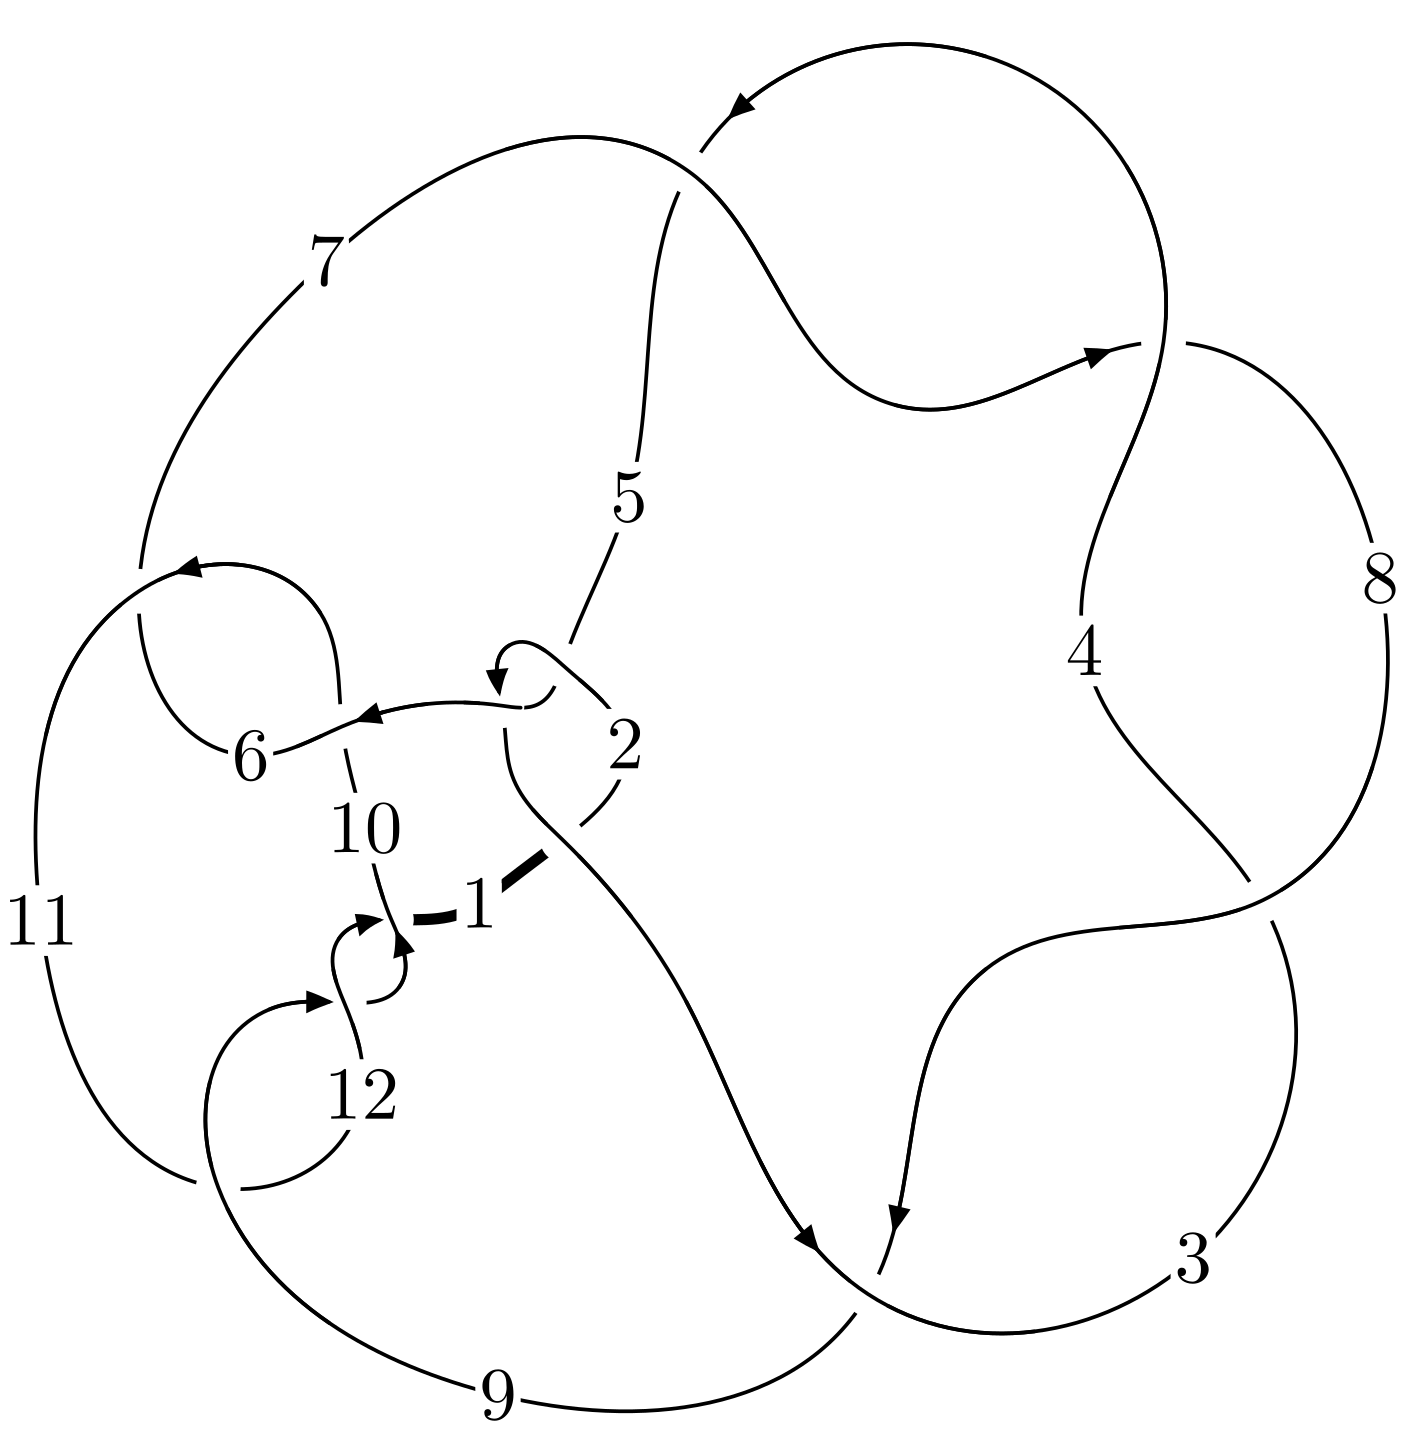
\includegraphics[width=112pt]{../../../GIT/diagram.site/Diagrams/png/2543_12n_0454.png}\\
\ \ \ A knot diagram\footnotemark}&
\allowdisplaybreaks
\textbf{Linearized knot diagam} \\
\cline{2-2}
 &
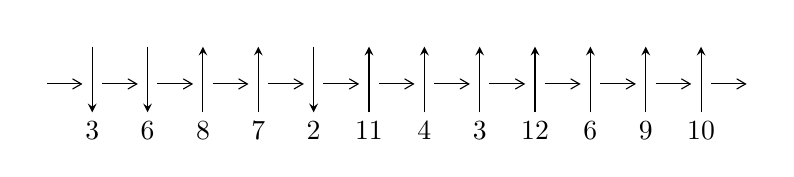
\begin{tikzpicture}[x=20pt, y=17pt]
	% nodes
	\node (C0) at (0, 0) {};
	\node (C1) at (1, 0) {};
	\node (C1U) at (1, +1) {};
	\node (C1D) at (1, -1) {3};

	\node (C2) at (2, 0) {};
	\node (C2U) at (2, +1) {};
	\node (C2D) at (2, -1) {6};

	\node (C3) at (3, 0) {};
	\node (C3U) at (3, +1) {};
	\node (C3D) at (3, -1) {8};

	\node (C4) at (4, 0) {};
	\node (C4U) at (4, +1) {};
	\node (C4D) at (4, -1) {7};

	\node (C5) at (5, 0) {};
	\node (C5U) at (5, +1) {};
	\node (C5D) at (5, -1) {2};

	\node (C6) at (6, 0) {};
	\node (C6U) at (6, +1) {};
	\node (C6D) at (6, -1) {11};

	\node (C7) at (7, 0) {};
	\node (C7U) at (7, +1) {};
	\node (C7D) at (7, -1) {4};

	\node (C8) at (8, 0) {};
	\node (C8U) at (8, +1) {};
	\node (C8D) at (8, -1) {3};

	\node (C9) at (9, 0) {};
	\node (C9U) at (9, +1) {};
	\node (C9D) at (9, -1) {12};

	\node (C10) at (10, 0) {};
	\node (C10U) at (10, +1) {};
	\node (C10D) at (10, -1) {6};

	\node (C11) at (11, 0) {};
	\node (C11U) at (11, +1) {};
	\node (C11D) at (11, -1) {9};

	\node (C12) at (12, 0) {};
	\node (C12U) at (12, +1) {};
	\node (C12D) at (12, -1) {10};
	\node (C13) at (13, 0) {};

	% arrows
	\draw[->,>={angle 60}]
	(C0) edge (C1) (C1) edge (C2) (C2) edge (C3) (C3) edge (C4) (C4) edge (C5) (C5) edge (C6) (C6) edge (C7) (C7) edge (C8) (C8) edge (C9) (C9) edge (C10) (C10) edge (C11) (C11) edge (C12) (C12) edge (C13) ;	\draw[->,>=stealth]
	(C1U) edge (C1D) (C2U) edge (C2D) (C3D) edge (C3U) (C4D) edge (C4U) (C5U) edge (C5D) (C6D) edge (C6U) (C7D) edge (C7U) (C8D) edge (C8U) (C9D) edge (C9U) (C10D) edge (C10U) (C11D) edge (C11U) (C12D) edge (C12U) ;
	\end{tikzpicture} \\
\hhline{~~} \\& 
\textbf{Solving Sequence} \\ \cline{2-2} 
 &
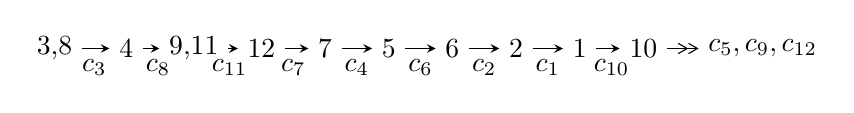
\begin{tikzpicture}[x=23pt, y=7pt]
	% node
	\node (A0) at (-1/8, 0) {3,8};
	\node (A1) at (1, 0) {4};
	\node (A2) at (33/16, 0) {9,11};
	\node (A3) at (25/8, 0) {12};
	\node (A4) at (33/8, 0) {7};
	\node (A5) at (41/8, 0) {5};
	\node (A6) at (49/8, 0) {6};
	\node (A7) at (57/8, 0) {2};
	\node (A8) at (65/8, 0) {1};
	\node (A9) at (73/8, 0) {10};
	\node (C1) at (1/2, -1) {$c_{3}$};
	\node (C2) at (3/2, -1) {$c_{8}$};
	\node (C3) at (21/8, -1) {$c_{11}$};
	\node (C4) at (29/8, -1) {$c_{7}$};
	\node (C5) at (37/8, -1) {$c_{4}$};
	\node (C6) at (45/8, -1) {$c_{6}$};
	\node (C7) at (53/8, -1) {$c_{2}$};
	\node (C8) at (61/8, -1) {$c_{1}$};
	\node (C9) at (69/8, -1) {$c_{10}$};
	\node (A10) at (11, 0) {$c_{5},c_{9},c_{12}$};

	% edge
	\draw[->,>=stealth]	
	(A0) edge (A1) (A1) edge (A2) (A2) edge (A3) (A3) edge (A4) (A4) edge (A5) (A5) edge (A6) (A6) edge (A7) (A7) edge (A8) (A8) edge (A9) ;
	\draw[->>,>={angle 60}]	
	(A9) edge (A10);
\end{tikzpicture} \\ 

\end{tabular} \\

\footnotetext{
The image of knot diagram is generated by the software ``\textbf{Draw programme}" developed by Andrew Bartholomew(\url{http://www.layer8.co.uk/maths/draw/index.htm\#Running-draw}), where we modified some parts for our purpose(\url{https://github.com/CATsTAILs/LinksPainter}).
}\phantom \\ \newline 
\centering \textbf{Ideals for irreducible components\footnotemark of $X_{\text{par}}$} 
 
\begin{align*}
I^u_{1}&=\langle 
-5.34392\times10^{24} u^{30}+1.20403\times10^{25} u^{29}+\cdots+2.13898\times10^{24} b-8.19442\times10^{25},\\
\phantom{I^u_{1}}&\phantom{= \langle  }-5.24612\times10^{24} u^{30}+1.21449\times10^{25} u^{29}+\cdots+2.13898\times10^{24} a-6.53057\times10^{25},\\
\phantom{I^u_{1}}&\phantom{= \langle  }u^{31}-2 u^{30}+\cdots+28 u+4\rangle \\
I^u_{2}&=\langle 
3 b- u-2,\;3 a+2 u+1,\;u^2+u+1\rangle \\
I^u_{3}&=\langle 
a u+3 b-4 a+2 u+1,\;2 a^2-3 a u+2 a+u-3,\;u^2+2\rangle \\
\\
I^v_{1}&=\langle 
a,\;b- v+2,\;v^2-3 v+1\rangle \\
\end{align*}
\raggedright * 4 irreducible components of $\dim_{\mathbb{C}}=0$, with total 39 representations.\\
\footnotetext{All coefficients of polynomials are rational numbers. But the coefficients are sometimes approximated in decimal forms when there is not enough margin.}
\newpage
\renewcommand{\arraystretch}{1}
\centering \section*{I. $I^u_{1}= \langle -5.34\times10^{24} u^{30}+1.20\times10^{25} u^{29}+\cdots+2.14\times10^{24} b-8.19\times10^{25},\;-5.25\times10^{24} u^{30}+1.21\times10^{25} u^{29}+\cdots+2.14\times10^{24} a-6.53\times10^{25},\;u^{31}-2 u^{30}+\cdots+28 u+4 \rangle$}
\flushleft \textbf{(i) Arc colorings}\\
\begin{tabular}{m{7pt} m{180pt} m{7pt} m{180pt} }
\flushright $a_{3}=$&$\begin{pmatrix}1\\0\end{pmatrix}$ \\
\flushright $a_{8}=$&$\begin{pmatrix}0\\u\end{pmatrix}$ \\
\flushright $a_{4}=$&$\begin{pmatrix}1\\- u^2\end{pmatrix}$ \\
\flushright $a_{9}=$&$\begin{pmatrix}u\\u\end{pmatrix}$ \\
\flushright $a_{11}=$&$\begin{pmatrix}2.45262 u^{30}-5.67789 u^{29}+\cdots+112.994 u+30.5312\\2.49834 u^{30}-5.62900 u^{29}+\cdots+123.421 u+38.3098\end{pmatrix}$ \\
\flushright $a_{12}=$&$\begin{pmatrix}2.40875 u^{30}-5.56826 u^{29}+\cdots+108.882 u+29.9698\\2.45447 u^{30}-5.51937 u^{29}+\cdots+119.309 u+37.7485\end{pmatrix}$ \\
\flushright $a_{7}=$&$\begin{pmatrix}- u\\u^3+u\end{pmatrix}$ \\
\flushright $a_{5}=$&$\begin{pmatrix}u^2+1\\- u^4-2 u^2\end{pmatrix}$ \\
\flushright $a_{6}=$&$\begin{pmatrix}0.185869 u^{30}-0.506326 u^{29}+\cdots+8.73363 u-0.480369\\0.954311 u^{30}-2.13631 u^{29}+\cdots+45.6943 u+14.8328\end{pmatrix}$ \\
\flushright $a_{2}=$&$\begin{pmatrix}1.20265 u^{30}-2.80559 u^{29}+\cdots+57.4529 u+14.8908\\-1.14984 u^{30}+2.60951 u^{29}+\cdots-55.1167 u-16.9723\end{pmatrix}$ \\
\flushright $a_{1}=$&$\begin{pmatrix}0.0528171 u^{30}-0.196085 u^{29}+\cdots+2.33621 u-2.08152\\-1.14984 u^{30}+2.60951 u^{29}+\cdots-55.1167 u-16.9723\end{pmatrix}$ \\
\flushright $a_{10}=$&$\begin{pmatrix}-0.871927 u^{30}+2.04345 u^{29}+\cdots-48.9524 u-11.3712\\2.44025 u^{30}-5.52900 u^{29}+\cdots+118.778 u+35.8466\end{pmatrix}$\\&\end{tabular}
\flushleft \textbf{(ii) Obstruction class $= -1$}\\~\\
\flushleft \textbf{(iii) Cusp Shapes $= \frac{40150014847740772034704846}{1604238713781269697683811} u^{30}-\frac{30333063294678849729282082}{534746237927089899227937} u^{29}+\cdots+\frac{642744006791888105510144570}{534746237927089899227937} u+\frac{616846322292496574153802580}{1604238713781269697683811}$}\\~\\
\newpage\renewcommand{\arraystretch}{1}
\flushleft \textbf{(iv) u-Polynomials at the component}\newline \\
\begin{tabular}{m{50pt}|m{274pt}}
Crossings & \hspace{64pt}u-Polynomials at each crossing \\
\hline $$\begin{aligned}c_{1}\end{aligned}$$&$\begin{aligned}
&u^{31}+34 u^{30}+\cdots+16249 u+361
\end{aligned}$\\
\hline $$\begin{aligned}c_{2},c_{5}\end{aligned}$$&$\begin{aligned}
&u^{31}+4 u^{30}+\cdots-17 u+19
\end{aligned}$\\
\hline $$\begin{aligned}c_{3},c_{4},c_{7}\\c_{8}\end{aligned}$$&$\begin{aligned}
&u^{31}+2 u^{30}+\cdots+28 u-4
\end{aligned}$\\
\hline $$\begin{aligned}c_{6},c_{10}\end{aligned}$$&$\begin{aligned}
&u^{31}+2 u^{30}+\cdots-36 u-36
\end{aligned}$\\
\hline $$\begin{aligned}c_{9},c_{11},c_{12}\end{aligned}$$&$\begin{aligned}
&u^{31}+6 u^{30}+\cdots+5 u+9
\end{aligned}$\\
\hline
\end{tabular}\\~\\
\newpage\renewcommand{\arraystretch}{1}
\flushleft \textbf{(v) Riley Polynomials at the component}\newline \\
\begin{tabular}{m{50pt}|m{274pt}}
Crossings & \hspace{64pt}Riley Polynomials at each crossing \\
\hline $$\begin{aligned}c_{1}\end{aligned}$$&$\begin{aligned}
&y^{31}-74 y^{30}+\cdots+131918441 y-130321
\end{aligned}$\\
\hline $$\begin{aligned}c_{2},c_{5}\end{aligned}$$&$\begin{aligned}
&y^{31}-34 y^{30}+\cdots+16249 y-361
\end{aligned}$\\
\hline $$\begin{aligned}c_{3},c_{4},c_{7}\\c_{8}\end{aligned}$$&$\begin{aligned}
&y^{31}+40 y^{30}+\cdots+272 y-16
\end{aligned}$\\
\hline $$\begin{aligned}c_{6},c_{10}\end{aligned}$$&$\begin{aligned}
&y^{31}+6 y^{30}+\cdots+2232 y-1296
\end{aligned}$\\
\hline $$\begin{aligned}c_{9},c_{11},c_{12}\end{aligned}$$&$\begin{aligned}
&y^{31}-20 y^{30}+\cdots+223 y-81
\end{aligned}$\\
\hline
\end{tabular}\\~\\
\newpage\flushleft \textbf{(vi) Complex Volumes and Cusp Shapes}
$$\begin{array}{c|c|c}  
\text{Solutions to }I^u_{1}& \I (\text{vol} + \sqrt{-1}CS) & \text{Cusp shape}\\
 \hline 
\begin{aligned}
u &= -0.150087 + 0.994909 I \\
a &= \phantom{-}0.49984 - 1.89088 I \\
b &= \phantom{-}1.130920 - 0.806791 I\end{aligned}
 & -3.71035 - 1.41787 I & \phantom{-}3.38804 + 1.32048 I \\ \hline\begin{aligned}
u &= -0.150087 - 0.994909 I \\
a &= \phantom{-}0.49984 + 1.89088 I \\
b &= \phantom{-}1.130920 + 0.806791 I\end{aligned}
 & -3.71035 + 1.41787 I & \phantom{-}3.38804 - 1.32048 I \\ \hline\begin{aligned}
u &= \phantom{-}0.949025 + 0.259341 I \\
a &= -0.072682 + 0.704869 I \\
b &= \phantom{-}0.582494 - 0.117627 I\end{aligned}
 & -3.71574 - 2.40842 I & \phantom{-}3.33618 + 2.66984 I \\ \hline\begin{aligned}
u &= \phantom{-}0.949025 - 0.259341 I \\
a &= -0.072682 - 0.704869 I \\
b &= \phantom{-}0.582494 + 0.117627 I\end{aligned}
 & -3.71574 + 2.40842 I & \phantom{-}3.33618 - 2.66984 I \\ \hline\begin{aligned}
u &= -0.761649 + 0.761026 I \\
a &= -0.101228 + 0.295647 I \\
b &= -0.778145 - 0.069572 I\end{aligned}
 & \phantom{-}1.17088 - 2.70519 I & \phantom{-}1.34730 + 7.26275 I \\ \hline\begin{aligned}
u &= -0.761649 - 0.761026 I \\
a &= -0.101228 - 0.295647 I \\
b &= -0.778145 + 0.069572 I\end{aligned}
 & \phantom{-}1.17088 + 2.70519 I & \phantom{-}1.34730 - 7.26275 I \\ \hline\begin{aligned}
u &= \phantom{-}0.801880 + 0.845490 I \\
a &= \phantom{-}0.192710 + 0.190905 I \\
b &= \phantom{-}1.308920 - 0.176651 I\end{aligned}
 & -5.44830 + 8.20678 I & \phantom{-}3.96431 - 6.25123 I \\ \hline\begin{aligned}
u &= \phantom{-}0.801880 - 0.845490 I \\
a &= \phantom{-}0.192710 - 0.190905 I \\
b &= \phantom{-}1.308920 + 0.176651 I\end{aligned}
 & -5.44830 - 8.20678 I & \phantom{-}3.96431 + 6.25123 I \\ \hline\begin{aligned}
u &= \phantom{-}0.518296 + 1.138380 I \\
a &= \phantom{-}0.075776 + 0.484959 I \\
b &= -0.478186 - 0.043766 I\end{aligned}
 & -8.10871 + 2.46499 I & \phantom{-0.000000 } 0 \\ \hline\begin{aligned}
u &= \phantom{-}0.518296 - 1.138380 I \\
a &= \phantom{-}0.075776 - 0.484959 I \\
b &= -0.478186 + 0.043766 I\end{aligned}
 & -8.10871 - 2.46499 I & \phantom{-0.000000 } 0\\
 \hline 
 \end{array}$$\newpage$$\begin{array}{c|c|c}  
\text{Solutions to }I^u_{1}& \I (\text{vol} + \sqrt{-1}CS) & \text{Cusp shape}\\
 \hline 
\begin{aligned}
u &= -0.239573 + 1.258650 I \\
a &= -0.049051 + 0.239996 I \\
b &= -0.174354 - 0.870729 I\end{aligned}
 & \phantom{-}3.35227 - 2.03069 I & \phantom{-}6.00000 + 0. I\phantom{ +0.000000I} \\ \hline\begin{aligned}
u &= -0.239573 - 1.258650 I \\
a &= -0.049051 - 0.239996 I \\
b &= -0.174354 + 0.870729 I\end{aligned}
 & \phantom{-}3.35227 + 2.03069 I & \phantom{-}6.00000 + 0. I\phantom{ +0.000000I} \\ \hline\begin{aligned}
u &= -0.049257 + 0.651330 I \\
a &= \phantom{-}0.031163 + 0.438228 I \\
b &= \phantom{-}0.636530 + 0.528351 I\end{aligned}
 & -1.02719 - 1.35876 I & \phantom{-}0.38562 + 5.54408 I \\ \hline\begin{aligned}
u &= -0.049257 - 0.651330 I \\
a &= \phantom{-}0.031163 - 0.438228 I \\
b &= \phantom{-}0.636530 - 0.528351 I\end{aligned}
 & -1.02719 + 1.35876 I & \phantom{-}0.38562 - 5.54408 I \\ \hline\begin{aligned}
u &= -0.01769 + 1.49068 I \\
a &= -1.84020 + 1.15884 I \\
b &= -2.05375 + 1.80415 I\end{aligned}
 & -4.97013 + 0.88940 I & \phantom{-0.000000 } 0 \\ \hline\begin{aligned}
u &= -0.01769 - 1.49068 I \\
a &= -1.84020 - 1.15884 I \\
b &= -2.05375 - 1.80415 I\end{aligned}
 & -4.97013 - 0.88940 I & \phantom{-0.000000 } 0 \\ \hline\begin{aligned}
u &= \phantom{-}0.146387 + 0.409089 I \\
a &= \phantom{-}0.10548 - 1.80116 I \\
b &= -1.016560 + 0.397771 I\end{aligned}
 & \phantom{-}1.43804 + 0.67860 I & \phantom{-}5.66172 + 1.82882 I \\ \hline\begin{aligned}
u &= \phantom{-}0.146387 - 0.409089 I \\
a &= \phantom{-}0.10548 + 1.80116 I \\
b &= -1.016560 - 0.397771 I\end{aligned}
 & \phantom{-}1.43804 - 0.67860 I & \phantom{-}5.66172 - 1.82882 I \\ \hline\begin{aligned}
u &= -0.333653\phantom{ +0.000000I} \\
a &= \phantom{-}4.41543\phantom{ +0.000000I} \\
b &= -0.313107\phantom{ +0.000000I}\end{aligned}
 & \phantom{-}7.50433\phantom{ +0.000000I} & \phantom{-}24.5590\phantom{ +0.000000I} \\ \hline\begin{aligned}
u &= \phantom{-}0.06381 + 1.68753 I \\
a &= \phantom{-}1.345990 + 0.237815 I \\
b &= \phantom{-}1.82999 - 0.04669 I\end{aligned}
 & -9.31296 - 0.73241 I & \phantom{-0.000000 } 0\\
 \hline 
 \end{array}$$\newpage$$\begin{array}{c|c|c}  
\text{Solutions to }I^u_{1}& \I (\text{vol} + \sqrt{-1}CS) & \text{Cusp shape}\\
 \hline 
\begin{aligned}
u &= \phantom{-}0.06381 - 1.68753 I \\
a &= \phantom{-}1.345990 - 0.237815 I \\
b &= \phantom{-}1.82999 + 0.04669 I\end{aligned}
 & -9.31296 + 0.73241 I & \phantom{-0.000000 } 0 \\ \hline\begin{aligned}
u &= \phantom{-}0.26352 + 1.68744 I \\
a &= \phantom{-}1.67424 + 0.15516 I \\
b &= \phantom{-}2.20381 - 0.62844 I\end{aligned}
 & -13.9459 + 12.3803 I & \phantom{-0.000000 } 0 \\ \hline\begin{aligned}
u &= \phantom{-}0.26352 - 1.68744 I \\
a &= \phantom{-}1.67424 - 0.15516 I \\
b &= \phantom{-}2.20381 + 0.62844 I\end{aligned}
 & -13.9459 - 12.3803 I & \phantom{-0.000000 } 0 \\ \hline\begin{aligned}
u &= -0.18187 + 1.70595 I \\
a &= -1.372120 - 0.010334 I \\
b &= -1.81881 - 0.60789 I\end{aligned}
 & -7.53329 - 6.21670 I & \phantom{-0.000000 } 0 \\ \hline\begin{aligned}
u &= -0.18187 - 1.70595 I \\
a &= -1.372120 + 0.010334 I \\
b &= -1.81881 + 0.60789 I\end{aligned}
 & -7.53329 + 6.21670 I & \phantom{-0.000000 } 0 \\ \hline\begin{aligned}
u &= -0.283237\phantom{ +0.000000I} \\
a &= -1.71193\phantom{ +0.000000I} \\
b &= -0.227764\phantom{ +0.000000I}\end{aligned}
 & \phantom{-}0.766548\phantom{ +0.000000I} & \phantom{-}14.0280\phantom{ +0.000000I} \\ \hline\begin{aligned}
u &= -0.03812 + 1.72844 I \\
a &= \phantom{-}1.237920 - 0.134015 I \\
b &= \phantom{-}1.67073 + 0.76279 I\end{aligned}
 & -13.51010 - 2.18010 I & \phantom{-0.000000 } 0 \\ \hline\begin{aligned}
u &= -0.03812 - 1.72844 I \\
a &= \phantom{-}1.237920 + 0.134015 I \\
b &= \phantom{-}1.67073 - 0.76279 I\end{aligned}
 & -13.51010 + 2.18010 I & \phantom{-0.000000 } 0 \\ \hline\begin{aligned}
u &= -0.260390\phantom{ +0.000000I} \\
a &= -0.560132\phantom{ +0.000000I} \\
b &= \phantom{-}2.58879\phantom{ +0.000000I}\end{aligned}
 & -0.450742\phantom{ +0.000000I} & \phantom{-}39.0360\phantom{ +0.000000I} \\ \hline\begin{aligned}
u &= \phantom{-}0.13397 + 1.76472 I \\
a &= -1.46619 - 0.05769 I \\
b &= -2.23420 - 0.13354 I\end{aligned}
 & -18.3679 + 5.2164 I & \phantom{-0.000000 } 0\\
 \hline 
 \end{array}$$\newpage$$\begin{array}{c|c|c}  
\text{Solutions to }I^u_{1}& \I (\text{vol} + \sqrt{-1}CS) & \text{Cusp shape}\\
 \hline 
\begin{aligned}
u &= \phantom{-}0.13397 - 1.76472 I \\
a &= -1.46619 + 0.05769 I \\
b &= -2.23420 + 0.13354 I\end{aligned}
 & -18.3679 - 5.2164 I & \phantom{-0.000000 } 0\\
 \hline 
 \end{array}$$\newpage\newpage\renewcommand{\arraystretch}{1}
\centering \section*{II. $I^u_{2}= \langle 3 b- u-2,\;3 a+2 u+1,\;u^2+u+1 \rangle$}
\flushleft \textbf{(i) Arc colorings}\\
\begin{tabular}{m{7pt} m{180pt} m{7pt} m{180pt} }
\flushright $a_{3}=$&$\begin{pmatrix}1\\0\end{pmatrix}$ \\
\flushright $a_{8}=$&$\begin{pmatrix}0\\u\end{pmatrix}$ \\
\flushright $a_{4}=$&$\begin{pmatrix}1\\u+1\end{pmatrix}$ \\
\flushright $a_{9}=$&$\begin{pmatrix}u\\u\end{pmatrix}$ \\
\flushright $a_{11}=$&$\begin{pmatrix}-\frac{2}{3} u-\frac{1}{3}\\\frac{1}{3} u+\frac{2}{3}\end{pmatrix}$ \\
\flushright $a_{12}=$&$\begin{pmatrix}-\frac{5}{3} u-\frac{1}{3}\\-\frac{2}{3} u+\frac{2}{3}\end{pmatrix}$ \\
\flushright $a_{7}=$&$\begin{pmatrix}- u\\u+1\end{pmatrix}$ \\
\flushright $a_{5}=$&$\begin{pmatrix}- u\\u+2\end{pmatrix}$ \\
\flushright $a_{6}=$&$\begin{pmatrix}- u\\u+1\end{pmatrix}$ \\
\flushright $a_{2}=$&$\begin{pmatrix}0\\- u\end{pmatrix}$ \\
\flushright $a_{1}=$&$\begin{pmatrix}- u\\- u\end{pmatrix}$ \\
\flushright $a_{10}=$&$\begin{pmatrix}-\frac{2}{3} u-\frac{1}{3}\\\frac{1}{3} u+\frac{2}{3}\end{pmatrix}$\\&\end{tabular}
\flushleft \textbf{(ii) Obstruction class $= 1$}\\~\\
\flushleft \textbf{(iii) Cusp Shapes $= \frac{4}{3} u+7$}\\~\\
\newpage\renewcommand{\arraystretch}{1}
\flushleft \textbf{(iv) u-Polynomials at the component}\newline \\
\begin{tabular}{m{50pt}|m{274pt}}
Crossings & \hspace{64pt}u-Polynomials at each crossing \\
\hline $$\begin{aligned}c_{1},c_{3},c_{4}\\c_{5}\end{aligned}$$&$\begin{aligned}
&u^2+u+1
\end{aligned}$\\
\hline $$\begin{aligned}c_{2},c_{7},c_{8}\end{aligned}$$&$\begin{aligned}
&u^2- u+1
\end{aligned}$\\
\hline $$\begin{aligned}c_{6},c_{10}\end{aligned}$$&$\begin{aligned}
&u^2
\end{aligned}$\\
\hline $$\begin{aligned}c_{9}\end{aligned}$$&$\begin{aligned}
&(u+1)^2
\end{aligned}$\\
\hline $$\begin{aligned}c_{11},c_{12}\end{aligned}$$&$\begin{aligned}
&(u-1)^2
\end{aligned}$\\
\hline
\end{tabular}\\~\\
\newpage\renewcommand{\arraystretch}{1}
\flushleft \textbf{(v) Riley Polynomials at the component}\newline \\
\begin{tabular}{m{50pt}|m{274pt}}
Crossings & \hspace{64pt}Riley Polynomials at each crossing \\
\hline $$\begin{aligned}c_{1},c_{2},c_{3}\\c_{4},c_{5},c_{7}\\c_{8}\end{aligned}$$&$\begin{aligned}
&y^2+y+1
\end{aligned}$\\
\hline $$\begin{aligned}c_{6},c_{10}\end{aligned}$$&$\begin{aligned}
&y^2
\end{aligned}$\\
\hline $$\begin{aligned}c_{9},c_{11},c_{12}\end{aligned}$$&$\begin{aligned}
&(y-1)^2
\end{aligned}$\\
\hline
\end{tabular}\\~\\
\newpage\flushleft \textbf{(vi) Complex Volumes and Cusp Shapes}
$$\begin{array}{c|c|c}  
\text{Solutions to }I^u_{2}& \I (\text{vol} + \sqrt{-1}CS) & \text{Cusp shape}\\
 \hline 
\begin{aligned}
u &= -0.500000 + 0.866025 I \\
a &= \phantom{-0.000000 } -0.577350 I \\
b &= \phantom{-}0.500000 + 0.288675 I\end{aligned}
 & \phantom{-}1.64493 - 2.02988 I & \phantom{-}6.33333 + 1.15470 I \\ \hline\begin{aligned}
u &= -0.500000 - 0.866025 I \\
a &= \phantom{-0.000000 -}0.577350 I \\
b &= \phantom{-}0.500000 - 0.288675 I\end{aligned}
 & \phantom{-}1.64493 + 2.02988 I & \phantom{-}6.33333 - 1.15470 I\\
 \hline 
 \end{array}$$\newpage\newpage\renewcommand{\arraystretch}{1}
\centering \section*{III. $I^u_{3}= \langle a u+3 b-4 a+2 u+1,\;2 a^2-3 a u+2 a+u-3,\;u^2+2 \rangle$}
\flushleft \textbf{(i) Arc colorings}\\
\begin{tabular}{m{7pt} m{180pt} m{7pt} m{180pt} }
\flushright $a_{3}=$&$\begin{pmatrix}1\\0\end{pmatrix}$ \\
\flushright $a_{8}=$&$\begin{pmatrix}0\\u\end{pmatrix}$ \\
\flushright $a_{4}=$&$\begin{pmatrix}1\\2\end{pmatrix}$ \\
\flushright $a_{9}=$&$\begin{pmatrix}u\\u\end{pmatrix}$ \\
\flushright $a_{11}=$&$\begin{pmatrix}a\\-\frac{1}{3} a u+\frac{4}{3} a-\frac{2}{3} u-\frac{1}{3}\end{pmatrix}$ \\
\flushright $a_{12}=$&$\begin{pmatrix}\frac{2}{3} a u+\frac{1}{3} a+\frac{4}{3} u+\frac{2}{3}\\\frac{1}{3} a u+\frac{2}{3} a+\frac{2}{3} u+\frac{1}{3}\end{pmatrix}$ \\
\flushright $a_{7}=$&$\begin{pmatrix}- u\\- u\end{pmatrix}$ \\
\flushright $a_{5}=$&$\begin{pmatrix}-1\\0\end{pmatrix}$ \\
\flushright $a_{6}=$&$\begin{pmatrix}-\frac{1}{3} a u+\frac{1}{3} a-\frac{7}{6} u-\frac{4}{3}\\-1\end{pmatrix}$ \\
\flushright $a_{2}=$&$\begin{pmatrix}-\frac{1}{3} a u+\frac{1}{3} a-\frac{7}{6} u-\frac{1}{3}\\-1\end{pmatrix}$ \\
\flushright $a_{1}=$&$\begin{pmatrix}-\frac{1}{3} a u+\frac{1}{3} a-\frac{7}{6} u-\frac{4}{3}\\-1\end{pmatrix}$ \\
\flushright $a_{10}=$&$\begin{pmatrix}- a u+a-\frac{3}{2} u-2\\-\frac{2}{3} a u+\frac{2}{3} a-\frac{1}{3} u-\frac{5}{3}\end{pmatrix}$\\&\end{tabular}
\flushleft \textbf{(ii) Obstruction class $= 1$}\\~\\
\flushleft \textbf{(iii) Cusp Shapes $= 4$}\\~\\
\newpage\renewcommand{\arraystretch}{1}
\flushleft \textbf{(iv) u-Polynomials at the component}\newline \\
\begin{tabular}{m{50pt}|m{274pt}}
Crossings & \hspace{64pt}u-Polynomials at each crossing \\
\hline $$\begin{aligned}c_{1},c_{5}\end{aligned}$$&$\begin{aligned}
&(u-1)^4
\end{aligned}$\\
\hline $$\begin{aligned}c_{2}\end{aligned}$$&$\begin{aligned}
&(u+1)^4
\end{aligned}$\\
\hline $$\begin{aligned}c_{3},c_{4},c_{7}\\c_{8}\end{aligned}$$&$\begin{aligned}
&(u^2+2)^2
\end{aligned}$\\
\hline $$\begin{aligned}c_{6},c_{11},c_{12}\end{aligned}$$&$\begin{aligned}
&(u^2+u-1)^2
\end{aligned}$\\
\hline $$\begin{aligned}c_{9},c_{10}\end{aligned}$$&$\begin{aligned}
&(u^2- u-1)^2
\end{aligned}$\\
\hline
\end{tabular}\\~\\
\newpage\renewcommand{\arraystretch}{1}
\flushleft \textbf{(v) Riley Polynomials at the component}\newline \\
\begin{tabular}{m{50pt}|m{274pt}}
Crossings & \hspace{64pt}Riley Polynomials at each crossing \\
\hline $$\begin{aligned}c_{1},c_{2},c_{5}\end{aligned}$$&$\begin{aligned}
&(y-1)^4
\end{aligned}$\\
\hline $$\begin{aligned}c_{3},c_{4},c_{7}\\c_{8}\end{aligned}$$&$\begin{aligned}
&(y+2)^4
\end{aligned}$\\
\hline $$\begin{aligned}c_{6},c_{9},c_{10}\\c_{11},c_{12}\end{aligned}$$&$\begin{aligned}
&(y^2-3 y+1)^2
\end{aligned}$\\
\hline
\end{tabular}\\~\\
\newpage\flushleft \textbf{(vi) Complex Volumes and Cusp Shapes}
$$\begin{array}{c|c|c}  
\text{Solutions to }I^u_{3}& \I (\text{vol} + \sqrt{-1}CS) & \text{Cusp shape}\\
 \hline 
\begin{aligned}
u &= \phantom{-0.000000 -}1.414210 I \\
a &= \phantom{-}0.618034 + 0.270091 I \\
b &= \phantom{-}0.618034 - 0.874032 I\end{aligned}
 & \phantom{-}2.30291\phantom{ +0.000000I} & \phantom{-}4.00000\phantom{ +0.000000I} \\ \hline\begin{aligned}
u &= \phantom{-0.000000 -}1.414210 I \\
a &= -1.61803 + 1.85123 I \\
b &= -1.61803 + 2.28825 I\end{aligned}
 & -5.59278\phantom{ +0.000000I} & \phantom{-}4.00000\phantom{ +0.000000I} \\ \hline\begin{aligned}
u &= \phantom{-0.000000 } -1.414210 I \\
a &= \phantom{-}0.618034 - 0.270091 I \\
b &= \phantom{-}0.618034 + 0.874032 I\end{aligned}
 & \phantom{-}2.30291\phantom{ +0.000000I} & \phantom{-}4.00000\phantom{ +0.000000I} \\ \hline\begin{aligned}
u &= \phantom{-0.000000 } -1.414210 I \\
a &= -1.61803 - 1.85123 I \\
b &= -1.61803 - 2.28825 I\end{aligned}
 & -5.59278\phantom{ +0.000000I} & \phantom{-}4.00000\phantom{ +0.000000I}\\
 \hline 
 \end{array}$$\newpage\newpage\renewcommand{\arraystretch}{1}
\centering \section*{IV. $I^v_{1}= \langle a,\;b- v+2,\;v^2-3 v+1 \rangle$}
\flushleft \textbf{(i) Arc colorings}\\
\begin{tabular}{m{7pt} m{180pt} m{7pt} m{180pt} }
\flushright $a_{3}=$&$\begin{pmatrix}1\\0\end{pmatrix}$ \\
\flushright $a_{8}=$&$\begin{pmatrix}v\\0\end{pmatrix}$ \\
\flushright $a_{4}=$&$\begin{pmatrix}1\\0\end{pmatrix}$ \\
\flushright $a_{9}=$&$\begin{pmatrix}v\\0\end{pmatrix}$ \\
\flushright $a_{11}=$&$\begin{pmatrix}0\\v-2\end{pmatrix}$ \\
\flushright $a_{12}=$&$\begin{pmatrix}2 v-1\\v-2\end{pmatrix}$ \\
\flushright $a_{7}=$&$\begin{pmatrix}v\\0\end{pmatrix}$ \\
\flushright $a_{5}=$&$\begin{pmatrix}1\\0\end{pmatrix}$ \\
\flushright $a_{6}=$&$\begin{pmatrix}v\\1\end{pmatrix}$ \\
\flushright $a_{2}=$&$\begin{pmatrix}- v+1\\-1\end{pmatrix}$ \\
\flushright $a_{1}=$&$\begin{pmatrix}- v\\-1\end{pmatrix}$ \\
\flushright $a_{10}=$&$\begin{pmatrix}-2 v+1\\-1\end{pmatrix}$\\&\end{tabular}
\flushleft \textbf{(ii) Obstruction class $= 1$}\\~\\
\flushleft \textbf{(iii) Cusp Shapes $= -6$}\\~\\
\newpage\renewcommand{\arraystretch}{1}
\flushleft \textbf{(iv) u-Polynomials at the component}\newline \\
\begin{tabular}{m{50pt}|m{274pt}}
Crossings & \hspace{64pt}u-Polynomials at each crossing \\
\hline $$\begin{aligned}c_{1},c_{2}\end{aligned}$$&$\begin{aligned}
&(u-1)^2
\end{aligned}$\\
\hline $$\begin{aligned}c_{3},c_{4},c_{7}\\c_{8}\end{aligned}$$&$\begin{aligned}
&u^2
\end{aligned}$\\
\hline $$\begin{aligned}c_{5}\end{aligned}$$&$\begin{aligned}
&(u+1)^2
\end{aligned}$\\
\hline $$\begin{aligned}c_{6},c_{9}\end{aligned}$$&$\begin{aligned}
&u^2- u-1
\end{aligned}$\\
\hline $$\begin{aligned}c_{10},c_{11},c_{12}\end{aligned}$$&$\begin{aligned}
&u^2+u-1
\end{aligned}$\\
\hline
\end{tabular}\\~\\
\newpage\renewcommand{\arraystretch}{1}
\flushleft \textbf{(v) Riley Polynomials at the component}\newline \\
\begin{tabular}{m{50pt}|m{274pt}}
Crossings & \hspace{64pt}Riley Polynomials at each crossing \\
\hline $$\begin{aligned}c_{1},c_{2},c_{5}\end{aligned}$$&$\begin{aligned}
&(y-1)^2
\end{aligned}$\\
\hline $$\begin{aligned}c_{3},c_{4},c_{7}\\c_{8}\end{aligned}$$&$\begin{aligned}
&y^2
\end{aligned}$\\
\hline $$\begin{aligned}c_{6},c_{9},c_{10}\\c_{11},c_{12}\end{aligned}$$&$\begin{aligned}
&y^2-3 y+1
\end{aligned}$\\
\hline
\end{tabular}\\~\\
\newpage\flushleft \textbf{(vi) Complex Volumes and Cusp Shapes}
$$\begin{array}{c|c|c}  
\text{Solutions to }I^v_{1}& \I (\text{vol} + \sqrt{-1}CS) & \text{Cusp shape}\\
 \hline 
\begin{aligned}
v &= \phantom{-}0.381966\phantom{ +0.000000I} \\
a &= \phantom{-0.000000 } 0 \\
b &= -1.61803\phantom{ +0.000000I}\end{aligned}
 & -0.657974\phantom{ +0.000000I} & -6.00000\phantom{ +0.000000I} \\ \hline\begin{aligned}
v &= \phantom{-}2.61803\phantom{ +0.000000I} \\
a &= \phantom{-0.000000 } 0 \\
b &= \phantom{-}0.618034\phantom{ +0.000000I}\end{aligned}
 & \phantom{-}7.23771\phantom{ +0.000000I} & -6.00000\phantom{ +0.000000I}\\
 \hline 
 \end{array}$$\newpage
\newpage\renewcommand{\arraystretch}{1}
\centering \section*{ V. u-Polynomials}
\begin{tabular}{m{50pt}|m{274pt}}
Crossings & \hspace{64pt}u-Polynomials at each crossing \\
\hline $$\begin{aligned}c_{1}\end{aligned}$$&$\begin{aligned}
&((u-1)^6)(u^2+u+1)(u^{31}+34 u^{30}+\cdots+16249 u+361)
\end{aligned}$\\
\hline $$\begin{aligned}c_{2}\end{aligned}$$&$\begin{aligned}
&((u-1)^2)(u+1)^4(u^2- u+1)(u^{31}+4 u^{30}+\cdots-17 u+19)
\end{aligned}$\\
\hline $$\begin{aligned}c_{3},c_{4}\end{aligned}$$&$\begin{aligned}
&u^2(u^2+2)^2(u^2+u+1)(u^{31}+2 u^{30}+\cdots+28 u-4)
\end{aligned}$\\
\hline $$\begin{aligned}c_{5}\end{aligned}$$&$\begin{aligned}
&((u-1)^4)(u+1)^2(u^2+u+1)(u^{31}+4 u^{30}+\cdots-17 u+19)
\end{aligned}$\\
\hline $$\begin{aligned}c_{6}\end{aligned}$$&$\begin{aligned}
&u^2(u^2- u-1)(u^2+u-1)^2(u^{31}+2 u^{30}+\cdots-36 u-36)
\end{aligned}$\\
\hline $$\begin{aligned}c_{7},c_{8}\end{aligned}$$&$\begin{aligned}
&u^2(u^2+2)^2(u^2- u+1)(u^{31}+2 u^{30}+\cdots+28 u-4)
\end{aligned}$\\
\hline $$\begin{aligned}c_{9}\end{aligned}$$&$\begin{aligned}
&((u+1)^2)(u^2- u-1)^3(u^{31}+6 u^{30}+\cdots+5 u+9)
\end{aligned}$\\
\hline $$\begin{aligned}c_{10}\end{aligned}$$&$\begin{aligned}
&u^2(u^2- u-1)^2(u^2+u-1)(u^{31}+2 u^{30}+\cdots-36 u-36)
\end{aligned}$\\
\hline $$\begin{aligned}c_{11},c_{12}\end{aligned}$$&$\begin{aligned}
&((u-1)^2)(u^2+u-1)^3(u^{31}+6 u^{30}+\cdots+5 u+9)
\end{aligned}$\\
\hline
\end{tabular}\newpage\renewcommand{\arraystretch}{1}
\centering \section*{ VI. Riley Polynomials}
\begin{tabular}{m{50pt}|m{274pt}}
Crossings & \hspace{64pt}Riley Polynomials at each crossing \\
\hline $$\begin{aligned}c_{1}\end{aligned}$$&$\begin{aligned}
&((y-1)^6)(y^2+y+1)(y^{31}-74 y^{30}+\cdots+1.31918\times10^{8} y-130321)
\end{aligned}$\\
\hline $$\begin{aligned}c_{2},c_{5}\end{aligned}$$&$\begin{aligned}
&((y-1)^6)(y^2+y+1)(y^{31}-34 y^{30}+\cdots+16249 y-361)
\end{aligned}$\\
\hline $$\begin{aligned}c_{3},c_{4},c_{7}\\c_{8}\end{aligned}$$&$\begin{aligned}
&y^2(y+2)^4(y^2+y+1)(y^{31}+40 y^{30}+\cdots+272 y-16)
\end{aligned}$\\
\hline $$\begin{aligned}c_{6},c_{10}\end{aligned}$$&$\begin{aligned}
&y^2(y^2-3 y+1)^3(y^{31}+6 y^{30}+\cdots+2232 y-1296)
\end{aligned}$\\
\hline $$\begin{aligned}c_{9},c_{11},c_{12}\end{aligned}$$&$\begin{aligned}
&((y-1)^2)(y^2-3 y+1)^3(y^{31}-20 y^{30}+\cdots+223 y-81)
\end{aligned}$\\
\hline
\end{tabular}
\vskip 2pc
\end{document}